\chapter{Evaluation}

The intention behind this work has been to develop an interactive visualization that effectively portrays the MS-PROD model and its implications.  We conducted two types of evaluations to determine which design alternatives were best for conveying this information: a formal evaluation of the arcs with novice users and an informal evaluation with expert users.  These two evaluations and the resulting findings are described in detail below. 

\section{Formal Evaluation of Dynamic Arcs}

We were interested in how different visualization alternatives enhance a user's understanding of the complex relationships between the fish species and the effects of those relationships.  In other words, is there a benefit to using dynamic, animated arcs---the most complicated representation of the relationships---over another method or even displaying no arcs at all?  To investigate this question, we designed and conducted a user study to measure the performance of different arc depiction alternatives.  The experimental conditions were as follows:

\begin{enumerate}[(A)]
\item No arcs
\item Static arcs
\item Dynamic arcs without animation
\item Dynamic arcs with animation
\end{enumerate}

Our hypothesis was that the Condition A would be the least effective, as it requires the user to guess why indirect or unexpected changes in biomass occurred since no arcs are drawn.  We also hypothesized that Condition C and Condition D would be more effective than Condition B, because dynamic arcs filter to show the relevant information, while static arcs show all information at once which could be overwhelming.  Finally, we hypothesized that Condition D would be at least slightly more effective than Condition C, since there are more visual cues for directionality with the animated arcs versus the non-animated arcs.

\subsection{Method}

The study was conducted at a screened-off table in a student union building at the University of New Hampshire.  A paid undergraduate research assistant conducted the study and responses from the study were graded by two paid undergraduate research assistants.

The research assistant conducting the experiment explained the MS-PROD model and our visualization to the participants, and showed a training example before leaving the participant to the experiment.  Each participant conducted the experiment task for only one of the four conditions.  Explanations and training phases were tailored according to the experimental condition---i.e., arcs were explained only for conditions B, C, and D; the meaning of dynamic arcs were explained only for conditions C and D.  Feedback about the quality of the participant's answers was given only during the training phase.  A single experiment lasted approximately fifteen minutes.

\subsection{Apparatus}

We conducted the experiment using a standard Dell laptop with an extra Dell monitor.  The window with the model visualization was maximized on the extra screen, while the window with the experiment questions was maximized on the laptop screen.  Participants used the mouse to interact with the model visualization and recorded their answers using the laptop keyboard.

\subsection{Participants}

There were 80 participants who took part in the study, all of which were recruited by a poster affixed to the backside of the privacy screen.  They could have been undergraduate or graduate students; we only required that participants had to be at least 18 years of age.  Participants were voluntary and were compensated with a pack of pens or a notebook.  They were required to read and sign an IRB consent form before participating in the study, shown in Appendix~\ref{sec:irbConsent}.

\subsection{Task}

Initially, all fishing effort sliders were set to the value of one.  Participants were instructed to increase or decrease the fishing effort of a specific functional group---e.g., \textit{``Using the sliders, double the harvest effort on elasmobranchs.''}  An example of this type of instructional window as it appeared to participants is shown in Figure~\ref{fig:eval_inst}.

\begin{figure}[h]
	\centering
	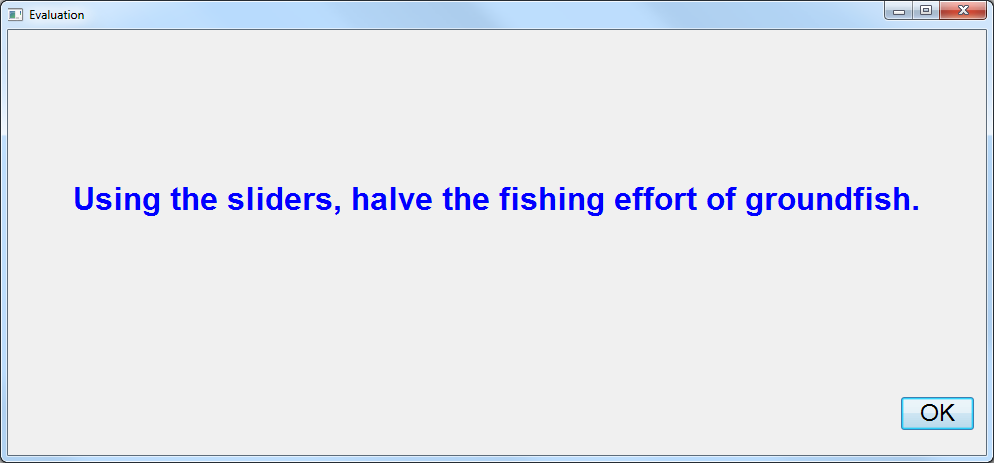
\includegraphics[width=0.5\textwidth]{figures/png/eval_instr.png}
	\caption{An instructional window in the evaluation which guides the participant.}
	\label{fig:eval_inst}
\end{figure}

Next, the participants were asked to answer one or more questions of the form, ``\textit{What was the effect on (fish species)?}''  E.g., \textit{``What was the effect on haddock?''}  All questions, as well as their answers, can be seen in Appendix~\ref{sec:questions}, grouped together by instruction.  %The questions were designed so that sometimes the fish species was a member of the function group for which the effort was just adjusted, while other times the fish species was not a member of that functional group.

Users answered this ``What\ldots?'' question with one of five options from a drop-down menu:
\begin{itemize}
\item \textit{Increased a lot}
\item \textit{Increased a little}
\item \textit{Stayed about the same}
\item \textit{Decreased a little}
\item \textit{Decreased a lot}
\end{itemize}
An example of the evaluation window as it appeared to users is shown in Figure~\ref{fig:eval_what}.

%\begin{figure}[h]
%	\centering
%	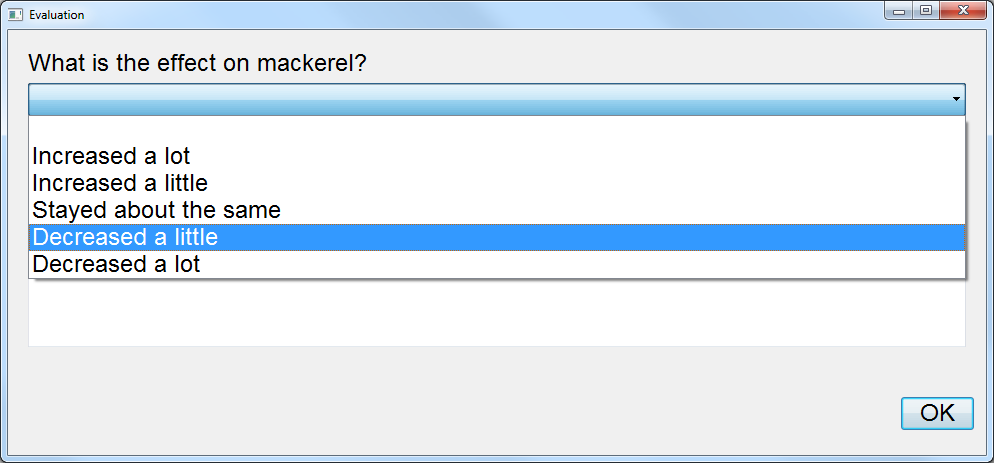
\includegraphics[width=0.48\textwidth]{figures/png/eval_what.png}
%	\caption{An example of evaluation window where users recorded their answers to the ``What\ldots?'' questions.}
%	\label{fig:eval_what}
%\end{figure}



\begin{figure}
\centering

\subfigure[The drop-down for selecting ``What\ldots?'' answers.]{\label{fig:eval_what}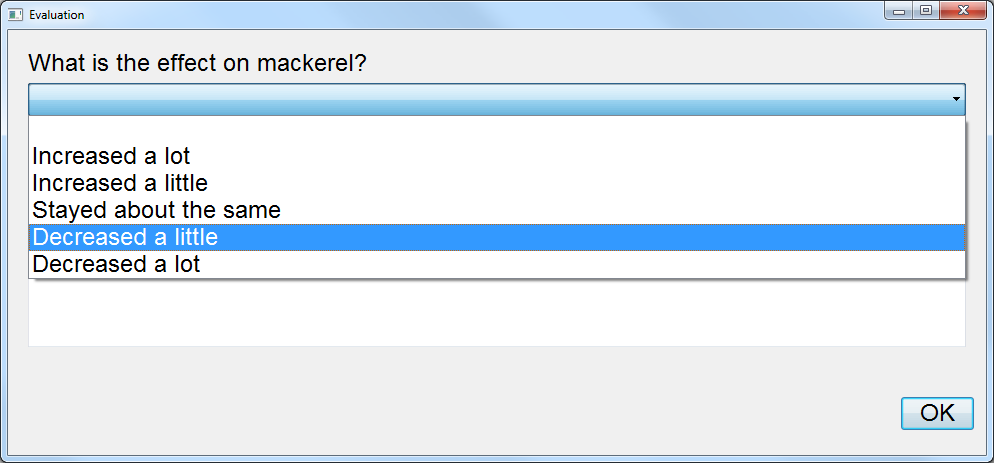
\includegraphics[width=0.48\textwidth]{figures/png/eval_what.png}} 
\subfigure[The text box for entering ``Why?'' answers.]{\label{fig:eval_why}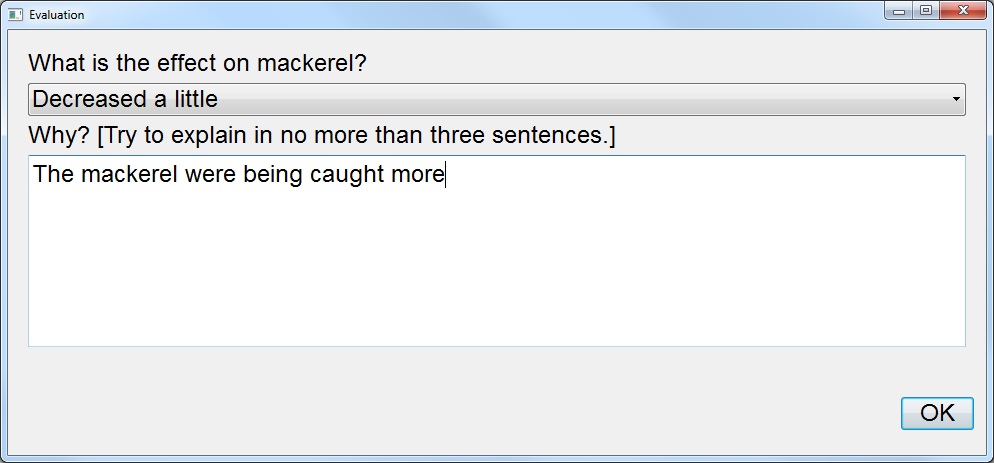
\includegraphics[width=0.48\textwidth]{figures/png/eval_why.png}}

	\caption{Examples of the windows where participants entered answers.}
	\label{fig:eval}
\end{figure}




Finally, the user was asked, ``\textit{Why? [Try to explain in no more than three sentences.]}''  A large text box was provided for the participant to type a response.  This is shown in Figure~\ref{fig:eval_why}. If this question was the last question in its set, then the sliders were all reset to one and a new instruction was given for the next set of questions until all questions were answered. 

%\begin{figure}[h]
%	\centering
%	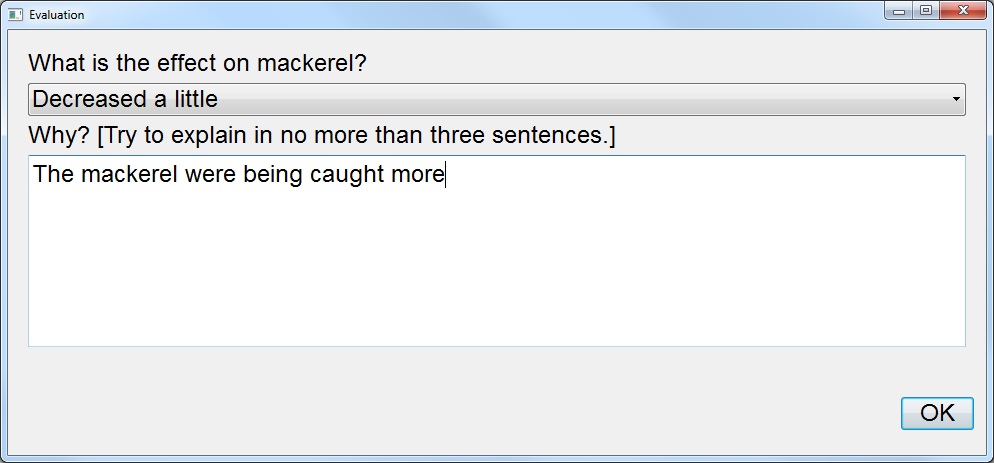
\includegraphics[width=0.48\textwidth]{figures/png/eval_why.png}
%	\caption{An example of evaluation window where users recorded their answers to the ``Why?'' questions.}
%	\label{fig:eval_why}
%\end{figure}

The questions were designed to fit in one of two difficulty categories:
\begin{itemize}
\item First-order
\item Higher-order
\end{itemize}

First-order questions asked about a fish species whose biomass changed directly as a result of increased or decreased harvest effort.  In other words, the fish was a member of the functional group whose harvest effort was changed and either (a) its biomass decreased due to increased harvest effort or (b) its biomass increased due to decreased harvest effort---e.g.,  increase harvest on A $\rightarrow$ biomass of A decreases.  There were three questions of this type.

Higher-order questions concerned a fish species whose biomass changed from a second-order or third-order effect.  In this case, the fish may or may not have been a member of the functional group for which the fishing effort changed.  If the fish was a member of the functional group, then perhaps its biomass did not change as expected because of the effects of competition or predation with other members of the functional group.  If the fish was not a member of the functional group for which fishing effort changed, then its biomass may have changed because of competition or predation with a member of that functional group---e.g., increase harvest on A $\rightarrow$ biomass of A decreases $\rightarrow$ biomass of B increases because A eats B.  More complex explanations involving several inter-species relationships are also possible---e.g., increase harvest on A $\rightarrow$ biomass of A decreases $\rightarrow$ biomass of B increases because A eats B $\rightarrow$ biomass of C decreases because B eats C.  There were four higher-order questions. 

In total, there were three instructions for adjusting the harvest effort and seven questions.  All participants were given the same instructions and asked the same questions in the same order, regardless of condition.

\subsection{Results}

\begin{figure}
\centering

\subfigure[``What\ldots?'' scores.]{\label{fig:resultsWhat}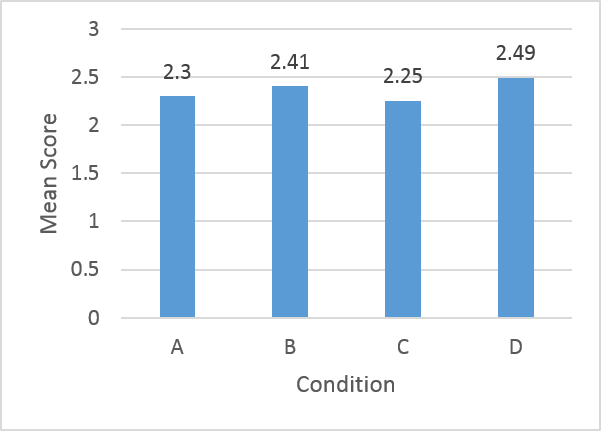
\includegraphics[width=0.32\textwidth]{figures/png/results_what.png}} 
\subfigure[First-order ``Why?'' scores.]{\label{fig:resultsWhy1}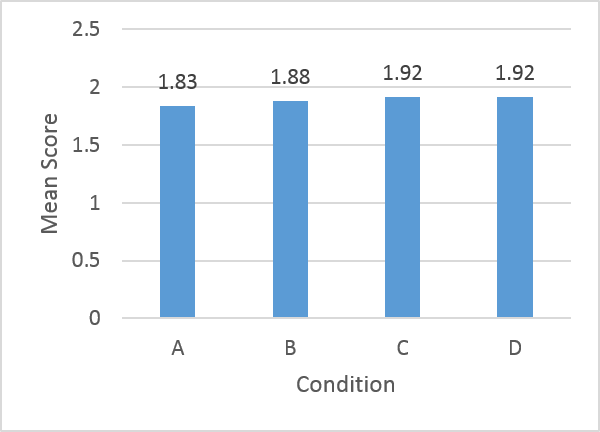
\includegraphics[width=0.32\textwidth]{figures/png/results_why1.png}}
\subfigure[Higher-order ``Why?'' scores.]{\label{fig:resultsWhy23}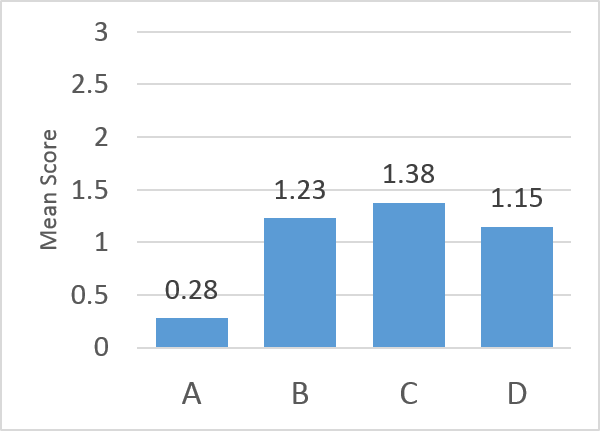
\includegraphics[width=0.32\textwidth]{figures/png/results_why23.png}}  

	\caption[Results of the formal evaluation, shown as mean scores graphed by condition.]{Results of the formal evaluation, shown as mean scores graphed by condition.  Scores were assigned on a scale from 0 to 3.}
	\label{fig:results}
\end{figure}

The answers to the questions of the evaluation were graded by two undergraduate graders on a scale of 0 (i.e., completely wrong) to 3 (i.e., completely correct), with partial points allowed.  The average of the two scores was taken and these averages were used in our analyses.  The correlation coefficient (Pearson's $r$) between the scores assigned by each grader was 0.744.

The summarized results of our evaluation can be found in Figure~\ref{fig:results}, where mean scores are shown by condition.  For our analyses, we divided the questions into three categories:
\begin{enumerate}
\item ``What\ldots?'' questions
\item First-order ``Why?'' questions
\item Higher-order ``Why?'' questions
\end{enumerate}
Separate ANOVAs (analysis of variance) were run with Tukey HSD (Honestly Significant Differences) tests for each of these three types of questions.  There were no significant differences between the four conditions for the seven ``What\ldots?'' questions and the three first-order ``Why?'' questions.    However, there was a significant effect for the four conditions with the higher-order ``Why?'' questions, shown by $([F(1, 76] = 12.6; p < 0.001)$ and the HSD test, with no other significant differences (see Figure~\ref{fig:resultsWhy23}).

\begin{figure}[h]
	\centering
	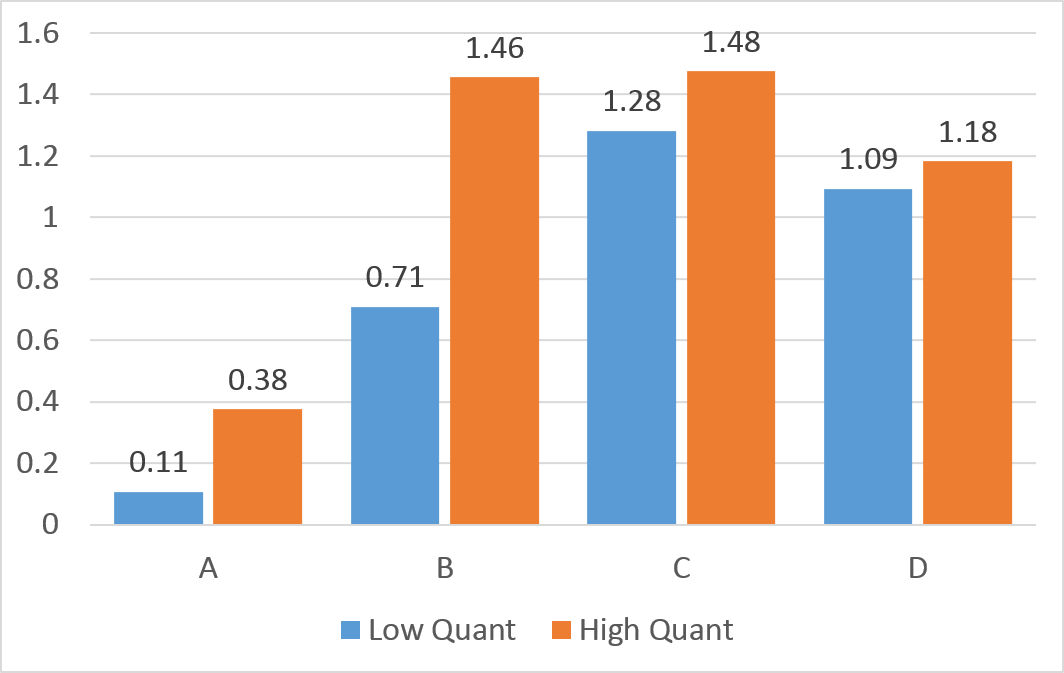
\includegraphics[width=0.85\textwidth]{figures/png/results_arts_science.png}
	\caption{Mean scores for arts versus sciences students for the higher-order ``Why?'' questions.}
	\label{fig:results_arts_science}
\end{figure}

Additional ANOVAs were run to look for effects of gender and whether the student was a ``science'' or liberal arts student.  We created a pseudo-category called ``science'' for participants who reported being part of the College of Engineering and Physical Sciences, College of Health and Human Services, College of Life Sciences, School of Marine Science and Ocean Engineering, Peter T. Paul College of Business and Economics, and the Thompson School of Applied Science; this included everyone except for participants from the College of Liberal Arts.  The gender and ``science'' versus liberal arts factors showed no significant effect on the higher-order ``Why?'' questions according to our analyses.  However, despite this, the effect for ``science'' versus liberal arts approached significance; the effects of this are illustrated in Figure~\ref{fig:results_arts_science}.  %The mean for science students in Condition A was over three times the mean for liberal arts students, while the gap was smaller for the other conditions.  This could possibly suggest that science students have a small advantage because they are used to analyzing time series in their classes, which helped them with the worst depiction of the inter-species relationships.

\subsection{Discussion}

Our results strongly suggest that using either static or dynamic arcs is better than using no arcs at all for asking more difficult (i.e., higher-order) questions about the complex, underlying relationships between the species.  The type of causal relationship depiction did not matter as much when it came to simpler (i.e., ``What\ldots?'' and first-order ``Why?'') questions.  For the ``What\ldots?'' questions, this is not surprising, as these questions were concerned with reading a change in a time series chart, for which the inter-species relationships were totally irrelevant.  Similarly, the first-order ``Why?'' questions involved direct effects of the changes in fishing effort, so understanding of the inter-species relationships was unnecessary.  Only the higher-order questions involved the competition and/or predation relationships, leading to a significance to the presence or absence of arcs.

Though the difference in mean score between ``science'' and liberal arts students, shown in Figure~\ref{fig:results_arts_science}, was not significant, it is interesting.  In Condition A (no arcs), the mean for science students was over three times the mean for liberal arts students.  This could possibly suggest that ``science'' students have more experience with quantitative analysis and reasoning, therefore they were able to perform better in the absence of arcs.  The gap narrowed in the other conditions; under Condition B (static arcs), ``science'' students had scores over twice as high as the liberal arts students on average, while the means were similar in Conditions C (dynamic arcs) and D (animated and dynamic arcs).  Again, there was not enough significance, so no conclusions should be drawn, but this may imply that dynamic arcs enabled liberal arts students to produce higher quality answers.  Perhaps an evaluation with more participants would produce a significant result concerning the type of student.

\section{Informal Evaluations}

%Originally, we had intended to conduct semi-structured interviews with expert users such as the original author models and fishery managers where we would ask the users to rate each alternative depiction of the different features.  However, we determined that would be a long and perhaps tedious task for each participant given the number of different depictions.  Therefore,
We interviewed three expert users in an informal environment in order to determine their preferences of the alternative depiction of the different features.  The informal interviews consisted of explaining and demonstrating the visualization to the participants and asking them to describe which alternative depictions they prefer, if any, and why.  Overall, the expert users who participated in the informal evaluations liked the visualization in general, particularly the dynamic, animated arcs.  More detailed findings of these informal evaluations are below; the comments were reconstructed from notes made in the meetings.

\subsection{Michael Fogerty and Robert Gamble} %Dr Fogerty

Dr.\ Michael Fogerty and Robert Gamble---members of the NOAA's National Marine Fisheries Services (NMFS) in Woods Hole, MA---are the original authors of the MS-PROD model with Jason Link.  We presented a prototype of the visualization in August 2013 and a more finalized visualization in January 2014.  The two of them have been pleased with the visualization.

Before we developed our visualization, they were using Microsoft Excel spreadsheets to graph the CSV output of the model after each run.  They reacted positively to the abilities to (a) change fishing effort parameters and see an instantaneous result and (b) easily perceive differences between forecasts that resulted from changes in fishing effort.  Dr.\ Fogerty suggested that the user should be able to set the baseline forecast at any moment, which we implemented.  Mr.\ Gamble expressed interest in keeping all alternative depictions in the final visualization, as he liked the ability to toggle between the various options.  He said he could see himself using the small multiples view to understand the relationships between the species, while he might use the four-panel view to prepare figures for future publications.

The feature that Dr.\ Fogerty and Mr.\ Gamble have been most enthusiastic about is the dynamic, animated arcs.  This feature was first demonstrated at a NMFS meeting on January 24, 2014.  Other members in attendance were also excited about the dynamic, animated arcs.  Mr.\ Gamble expressed that even sometimes he can become confused about the counter-intuitive effects of the underlying relationships and must refer to the predation and competition matrices in the original parameter file to understand them; the dynamic arcs eliminate the need for this extra work by making the relevant relationships more obvious.  Members in attendance were very interested in the potential to adapt the visualization to other models.  Furthermore, they believed the visualization would allow them to make convincing arguments to fishery managers or other import decision makers to use the MS-PROD model or similar models.

Dr.\ Michael Fogerty and Robert Gamble have been further developing the MS-PROD model to include types of fishing (e.g., bottom trawl, midwater trawl, long lines, dredges) with different catchabilities for each pair of fish species and fishing type.  They have also introduced climate factors (e.g., average sea floor temperature).  They have expressed interest in incorporating these new factors into the visualization, as well as the ability to include more species and/or functional groups.  Furthermore, Dr.\ Fogerty is interested in developing a version of the visualization that is compatible with browsers for usage by the general public.  However, Gamble expressed reluctance to use the actual names of fish species because this could result in over-interpretation of the results and suggested that generic names like ``Elasmobranch 1'' and ``Elasmobranch 2'' be used.

In general, Dr.\ Fogerty and Mr.\ Gamble were satisfied with the quality of the visualization.  Mr.\ Gamble said that he was not sure how to express what he wanted in a visualization when our collaboration began, but he saw what he had originally envisioned when he saw the finalized visualization.  

\subsection{David Goethel}

On April 1, 2014, we conducted an informal interview with David Goethel.  David Goethel is a biologist and fisherman based out of Hampton, New Hampshire, who has advised several state and federal fishery management boards and served on the New England Fishery Management Council.  As a fisherman, he catches all ten of the species used in the MS-PROD model throughout the year, as well as others.  He has been an advocate for moving toward a more sustainable approach to fishery management and is interested in models which can help illustrate that change is necessary.  

Mr.\ Goethel found both the small multiple and four panel views useful.  He did not have a preference over either view and said that he might choose which one to use depending on his intended audience or what he was investigating in the model.  Similarly, he said he liked all options for uncertainty visualization and would choose based on his audience; he might use error bands when presenting to the general public, but use box plots for fishery managers.  He had previously believed that stock assessments should be presented more like hurricane tracks, with multiple forecasts to show multiple opinions, therefore he found the range of forecasts shown in the uncertainty view to be particularly helpful.

As for the different depictions of change, Mr.\ Goethel preferred the blended, shaded area between the two forecasts over instantaneous change only or the dotted line for the previous forecast.  He said he would always use the blended option because it was more informative.  For understanding the relationships between fish, he preferred the dynamic, animated arc over all other options.  This option allows the user to ``follow the flow [of the relationships] more easily,'' while he found it ``harder to see the conclusion'' of the effects of the harvest without animation.  He was excited to see a visualization of these relationships because they can be counter-intuitive even to someone with as much experience as him.

Overall, Mr.\ Goethel was interested in the model, saying that its visualization would help to convince people that more complex models like MS-PROD are necessary.  He said fishery managers typically prefer single species models and make decisions for ten-year periods.  However, Mr.\ Goethel finds it important to considering multiple species as well as other factors and to think about management for longer time periods, like MS-PROD.  He said that MS-PROD ``might reflect reality more,'' and our visualization might help to persuading managers of this.  He said he recommended restricting access of the model to scientific community only for now and waiting before presenting it to the general public to avoid unexperienced users from drawing incorrect conclusions.
